%% Based on a TeXnicCenter-Template by Gyorgy SZEIDL.
%%%%%%%%%%%%%%%%%%%%%%%%%%%%%%%%%%%%%%%%%%%%%%%%%%%%%%%%%%%%%

%----------------------------------------------------------
%
\documentclass[10pt,a4paper,answers]{exam}
%\documentclass[10pt,a4paper]{exam}
%
%----------------------------------------------------------
% This is a sample document for the standard LaTeX Book Class
% Class options
%       --  Body text point size:
%                        10pt (default), 11pt, 12pt
%       --  Paper size:  letterpaper (8.5x11 inch, default)
%                        a4paper, a5paper, b5paper,
%                        legalpaper, executivepaper
%       --  Orientation (portrait is the default):
%                        landscape
%       --  Printside:   oneside, twoside (default)
%       --  Quality:     final(default), draft
%       --  Title page:  titlepage, notitlepage
%       --  Columns:     onecolumn (default), twocolumn
%       --  Start chapter on left:
%                        openright(no, default), openany
%       --  Equation numbering (equation numbers on right is the default):
%                        leqno
%       --  Displayed equations (centered is the default):
%                        fleqn (flush left)
%       --  Open bibliography style (closed bibliography is the default):
%                        openbib
% For instance the command
%          \documentclass[a4paper,12pt,reqno]{book}
% ensures that the paper size is a4, fonts are typeset at the size 12p
% and the equation numbers are on the right side.
%
\usepackage{multicol}
\usepackage{enumerate}
\usepackage{amsthm}
\usepackage{amsmath}%
\usepackage{amsfonts}%
\usepackage{amssymb}%
\usepackage{graphicx}
	\graphicspath{ {images/} }
\usepackage[pdftex]{epsfig}
\usepackage{booktabs} % Better horizontal rules
\usepackage{listings}
\usepackage{hyperref}
\usepackage{float} 



\usepackage{textcomp}
\usepackage{listings}
\lstset{upquote=true}
\lstset{basicstyle = \ttfamily,columns=fullflexible}


\usepackage{prftree}
\usepackage{listings}
\usepackage{xcolor}
\definecolor{OliveGreen}{RGB}{100,184,108}
\definecolor{NavyBlue}{RGB}{0,0,108}
\definecolor{ProcessBlue}{RGB}{0,0,108}

\newtheorem{proposition}{Proposition}
\newtheorem{definition}{Definition}

% Setup TikZ

\usepackage{tikz}
\usetikzlibrary{arrows}
\tikzset{
    % Define arrow style
    arrow/.style={
           ->,}
}

\begin{document}
\begin{center}
{\sf\large \bf BT5110}
\end{center}
\begin{center}
{\sf\large \bf Test 1}
\end{center}
\vspace{2.3cm}

\underline{{\large{\sf INSTRUCTIONS}}}

\begin{enumerate}
\item This assessment {\bf starts at 18:40}.
\item This assessment {\bf ends at 20:30}.
\item The {\bf maximum mark is 25.}
\item This is an {\bf open book, open computer, and open Internet assessment}.
\item You are not allowed to communicate with anyone but  members of the teaching team. Shall you use any external source of information make sure that you include a reference to the source in your answer (e.g. the URL).
\item Any student who is alleged to have committed or attempted to commit, or caused or attempted to cause any other person to commit any of the following offences: plagiarism, giving or receiving unauthorised assistance in academic work, or other forms of academic dishonesty, may be subject to disciplinary proceedings.

\item{\bf Download this question paper and the template answer file}:
\begin{itemize}
    \item  ``\verb+test1.pdf+'',
    \item  ``\verb+answers.sql+'',
\end{itemize}
from the Luminus directory:

``\verb+Files > Tests > Test 1+''.
\item {\bf Download the following files}:
\begin{itemize}
    \item ``\verb+app.sql+'',
    \item ``\verb+appfunctionality.sql+'',
    \item ``\verb+available.sql+'',
    \item ``\verb+country.sql+'',
    \item ``\verb+functionality.sql+'', and
    \item ``\verb+store.sql+''.
\end{itemize}
  from the Luminus directory:

``\verb+Files > Cases > Covid19+''.

\item {\bf Write your  student number} in the corresponding section of the file ``\verb+answers.sql+''.

\item {\bf Write  your answers} to the questions in the corresponding sections of the file ``\verb+answers.sql+''.

\item {\bf Within the 10 minutes following the end of the assessment, upload the file} ``\verb+answers.sql+'' to the Luminus directory:

``\verb+Files > Tests > Test 1 > Submissions+''.
\end{enumerate}
\vspace{1cm}

\pagebreak

\begin{questions} 
\question The European Commission Joint Research Centre maintains a data set of mobile applications (apps) published across the world to fight the COVID-19 crisis. We consider a simplified subset of the data set stored in a relational schema comprising six self-describing  tables.

Read the SQL data definition language code in the SQL files provided and explore the provided instances of the tables to understand the application. Notice that the table country is denormalised.

Prefer simple queries to nested queries, algebraic queries, and aggregate queries, in this order unless otherwise specified or strictly necessary. Do not use subqueries in the \verb+FROM+ clause unless otherwise specified or absolutely necessary. Do not create temporary tables, views, or stored functions and triggers unless otherwise specified or absolutely necessary. Your answers should be correct for the example database instance and for other instances of the same schema (for instance, new or updated apps,  stores, functionalities, etc.). Your SQL code must run on PostgreSQL version 13 and above.

\begin{parts} 
\part[3] (SQL) Print the names and ISO two letter codes of the different continents. The result should be similar to that in the table below in any order. 

\vspace{0.2cm}
\begin{center}
\begin{tabular}{|l|l|}
\hline
\hline
continent\_name  & continent\_code  \\ \hline
\hline
"Africa" &	"AF" \\ \hline
"Europe"	 & "EU" \\ \hline
"South America"	& "SA" \\ \hline
"Asia" & 	"AS" \\ \hline
"North America"	& "NA" \\ \hline
"Oceania" &	"OC" \\ \hline
"Antarctica"	& "AN" \\ \hline
\hline
\end{tabular}
\end{center}
\vspace{0.2cm}

\begin{solution}
\begin{lstlisting}
SELECT DISTINCT continent_name, continent_code 
FROM country;
\end{lstlisting}
\end{solution}


\part[3] (SQL) Find the contact tracing apps that are available in Europe and work for both iOS and Android operating systems. For each app, print  the name of the app (rename the column as ``\verb+app+'') and the name of the country (rename the column as ``\verb+country+'') in which the app is available. The result should be similar to that in the table below in any order. 

\vspace{0.2cm}
\begin{center}
\begin{tabular}{|l|l|}
\hline
\hline
app  & country  \\ \hline
\hline
"COVID-19.eus"&	"Spain, Kingdom of"\\ \hline
"Rakning C-19"	&"Iceland, Republic of"\\ \hline
"Stopp Corona"	&"Austria, Republic of"\\ \hline
"Corona-Warn-App"&	"Germany, Federal Republic of"\\ \hline
"Immuni"	&"Italy, Italian Republic"\\ \hline
"StopKorona!"	&"Macedonia, The Former Yugoslav Republic of"\\ \hline
"SwissCovid"	&"Switzerland, Swiss Confederation"\\ \hline
"ProteGO Safe"	&"Poland, Republic of"\\ \hline
"Apturi Covid Latvia – SPKC"&	"Latvia, Republic of"\\ \hline
"StopCovid France"	&"France, French Republic"\\ \hline
\hline
\end{tabular}
\end{center}
\vspace{0.2cm}

\begin{solution}
\begin{lstlisting}
SELECT  a.name as app, c.name as country
FROM appfunctionality a, available av, country c, store s1, store s2
WHERE a.name=av.name
AND av.country=c.code3
AND c.continent_name='Europe'
AND a.functionality = 'contact tracing'
AND a.name=s1.name
AND s1.os='iOS'
AND a.name=s2.name
AND s2.os='Android';
\end{lstlisting}
DISTINCT is redundant since the continent is specified.
\end{solution}
 
\part[3] (SQL) Find the names of the countries that are spanning over several continents. Use aggregate functions. The result should be similar to that in the table below in any order. 

\vspace{0.2cm}
\begin{center}
\begin{tabular}{|l|}
\hline
\hline
name\\ \hline
\hline
"Armenia, Republic of"\\ \hline
"Azerbaijan, Republic of"\\ \hline
"Cyprus, Republic of"\\ \hline
"Georgia"\\ \hline
"Kazakhstan, Republic of"\\ \hline
"Russian Federation"\\ \hline
"Turkey, Republic of"\\ \hline
"United States Minor Outlying Islands"\\ \hline
\hline
\end{tabular}
\end{center}
\vspace{0.2cm}

\begin{solution}
\begin{lstlisting}
SELECT c1.name
FROM country c1
GROUP BY c1.name
HAVING count(DISTINCT c1.continent_name) >1;
\end{lstlisting}
\end{solution}

\part[3] (SQL) Find the names of the countries that are spanning over several continents. This is the same query as (1.c) only do not use an aggregate query. The result should be similar to that in the table above in any order. 

\begin{solution}
\begin{lstlisting}
SELECT DISTINCT c1.name
FROM country c1, country c2
WHERE c1.name = c2.name 
AND c1.continent_name < c2.continent_name;
\end{lstlisting}
or
\begin{lstlisting}
SELECT DISTINCT * 
FROM (SELECT name
  FROM country c1
  EXCEPT ALL
  SELECT DISTINCT c1.name
  FROM country c1) 
AS cross_continent_countries;
\end{lstlisting}
Need to be careful here because you cannot assume all cross continent countries only span 2 continents, e.g., France has territory in all continents except Asia: Oceania (Tahiti), Africa (Reunion), N.America (St. Pierre \& Miqueion) and S.America (French Guiana).
\end{solution}

\part[3] (SQL) Find the names of the apps available in countries in Oceania that work for all recorded operating systems. The result should be similar to that in the table below in any order.  Make sure that your query produces the correct result in all possible database instances including when new apps with new operating systems are added (you may neither hardcode the operating systems as in Question 1.b nor the number of operating systems.)  Do not use an aggregate query.

\vspace{0.2cm}
\begin{center}
\begin{tabular}{|l|}
\hline
\hline
name\\ \hline
\hline
"TCC COVID Monitor"\\ \hline
"healthdirect"\\ \hline
"Coronavirus Australia"\\ \hline
"MyAus COVID-19"\\ \hline
"\#BeatCovid19Now"\\ \hline
"Bupa Aged Care Connect"\\ \hline
"NZ COVID Tracer"\\ \hline
"COVIDSafe"\\ \hline
\hline
\end{tabular}
\end{center}
\vspace{0.2cm}

\begin{solution}
\begin{lstlisting}
SELECT a.name
FROM app a, available av, country c
WHERE a.name = av.name 
AND av.country = c.code3
AND c.continent_name='Oceania'
AND NOT EXISTS (SELECT *
 FROM store s1
 WHERE 
 NOT EXISTS (SELECT * 
  FROM store s2
  WHERE s2.name = a.name
  AND s1.os = s2.os))
\end{lstlisting}

The following is not entirely satisfactory as a country may span over Oceania and another continent (USA and France have territories in Oceania etc.)

\begin{lstlisting}
SELECT  a.name
FROM app a, available av, country c, store s1
WHERE a.name=av.name
AND av.country=c.code3
AND a.name = s1.name
AND c.continent_name='Oceania'
GROUP BY a.name
HAVING COUNT(*) = (SELECT COUNT(DISTINCT s2.os) FROM store s2)
\end{lstlisting}
\end{solution}

\part[3] (SQL) Find the countries with the top 6 largest number of apps available (this is a dense ranking of the countries according to the number of apps). Print the names of the countries and the numbers of apps in descending order of the numbers of apps. The result should be similar to that in the table below. For full mark, make sure that your query produces the correct result for the top 7, 8 to 16 as well. Do not use ``\verb+RANK()+'', ``\verb+DENSE_RANK()+'', ``\verb+ROW_NUMBER()+'', window functions and partitions (although they  could be  better choices in this case.) Use ``\verb+GROUP BY+'', ``\verb+ORDER BY+'', and ``\verb+LIMIT+''. 

\vspace{0.2cm}
\begin{center}
\begin{tabular}{|l|l|}
\hline
\hline
name & count \\ \hline
\hline
"United States of America"	&65\\ \hline
"India, Republic of"	&52\\ \hline
"Mexico, United Mexican States"	&21\\ \hline
"Brazil, Federative Republic of"&	17\\ \hline
"Spain, Kingdom of"	&16\\ \hline
"United Kingdom of Great Britain \& Northern Ireland"	& 14\\ \hline
\hline
\end{tabular}
\end{center}
\vspace{0.2cm}

\begin{solution}
\begin{lstlisting}
SELECT c1.name, count(a1.name) as count
 FROM (SELECT DISTINCT c3.name, c3.code3 FROM country c3) AS c1 
    LEFT OUTER JOIN available a1 
    ON c1.code3 = a1.country
 GROUP BY c1.name
 	HAVING COUNT(a1.name) IN
( SELECT DISTINCT COUNT(a2.name) 
 FROM (SELECT DISTINCT c4.name, c4.code3 FROM country c4) AS c2 
    LEFT OUTER JOIN available a2 
    ON c2.code3 = a2.country
 GROUP BY c2.name
 ORDER BY count DESC
 LIMIT 6)
 ORDER BY count DESC;
\end{lstlisting}

One has to group by name and not by code3, because some code3 are null.

This following solution is almost correct but it counts countries spanning over two continents twice. RUS is in top 7, it should appear in top 10. 
\begin{lstlisting}
SELECT c1.code3, count(a1.name) as count
 FROM country c1 LEFT OUTER JOIN available a1 ON c1.code3 = a1.country
 GROUP BY c1.code3
 	HAVING COUNT(a1.name) IN
( SELECT DISTINCT COUNT(a2.name) 
 FROM country c2 LEFT OUTER JOIN available a2 ON c2.code3 = a2.country
 GROUP BY c2.code3
 ORDER BY count DESC
 LIMIT 6)
 ORDER BY count DESC;
\end{lstlisting}
This following solution is almost correct but misses the 0 counts. Test with top 16 (87 instead of 254 results).
\begin{lstlisting}
SELECT c1.name, count(a1.name) as count
 FROM country c1, available a1
 WHERE c1.code3 = a1.country
 GROUP BY c1.name
 	HAVING COUNT(a1.name) IN
( SELECT DISTINCT COUNT(a2.name) 
 FROM country c2, available a2 
 WHERE c2.code3 = a2.country
 GROUP BY c2.name
 ORDER BY count DESC
 LIMIT 6)
 ORDER BY count DESC;
\end{lstlisting}

The following answer is not correct. Try with top 8 and 10.
\begin{lstlisting}
SELECT c.name, COUNT(*) as count 
FROM available a, country c
WHERE c.code3=a.country
GROUP BY c.name
ORDER BY count 
DESC LIMIT 6
\end{lstlisting}
\end{solution}
\end{parts}


\pagebreak
\question\label{ques:er} Consider the  entity-relationship diagram in Figure 1 (omitted).

\begin{parts}
\part[5] Translate the entity-relationship diagram into SQL following the translation rules given in the lecture. Use ``\verb+TEXT+'' as the domain of the columns. Make sure that the design does not allow null values. The code should run for PostgreSQL version 13 and above (try it).
\begin{solution}
\begin{lstlisting}
CREATE TABLE E1S (
A TEXT UNIQUE NOT NULL,
B TEXT NOT NULL,
C TEXT,
D TEXT,
F TEXT NOT NULL,
G TEXT REFERENCES E2(G),
PRIMARY KEY (C, D));
\end{lstlisting}
or
\begin{lstlisting}
CREATE TABLE E1S (
A TEXT PRIMARY KEY,
B TEXT NOT NULL,
C TEXT NOT UNIQUE NOT NULL,
D TEXT NOT UNIQUE NOT NULL,
F TEXT NOT NULL,
G TEXT REFERENCES E2(G));
\end{lstlisting}

\begin{lstlisting}
CREATE TABLE E2 (
J TEXT ,
K TEXT NOT NULL,
G TEXT NOT PRIMARY KEY,
H TEXT NOT NOT NULL);
\end{lstlisting}


If the answer has three tables, for partial marks:
\begin{lstlisting}
CREATE TABLE E1 (
A TEXT UNIQUE NOT NULL,
B TEXT NOT NULL,
C TEXT,
D TEXT,
PRIMARY KEY (C, D));
\end{lstlisting}
or
\begin{lstlisting}
CREATE TABLE E1 (
A TEXT PRIMARY KEY,
B TEXT NOT NULL,
C TEXT NOT UNIQUE NOT NULL,
D TEXT NOT UNIQUE NOT NULL);
\end{lstlisting}

\begin{lstlisting}
CREATE TABLE E2 (
J TEXT ,
K TEXT NOT NULL,
G TEXT PRIMARY KEY,
H TEXT NOT NOT NULL);
\end{lstlisting}

\begin{lstlisting}
CREATE TABLE S (
C TEXT,
D TEXT,
F TEXT NOT NULL,
G TEXT REFERENCES E2(G),
FOREIGN KEY (C, D) REFERENCES E1(C, D),
PRIMARY KEY (C, D, G));
\end{lstlisting}
or
\begin{lstlisting}
CREATE TABLE S (
A TEXT REFERENCES E1(A),
F TEXT NOT NULL,
G TEXT REFERENCES E2(G),
PRIMARY KEY (C, A));
\end{lstlisting}

\end{solution}

\begin{figure}
	\begin{center}
		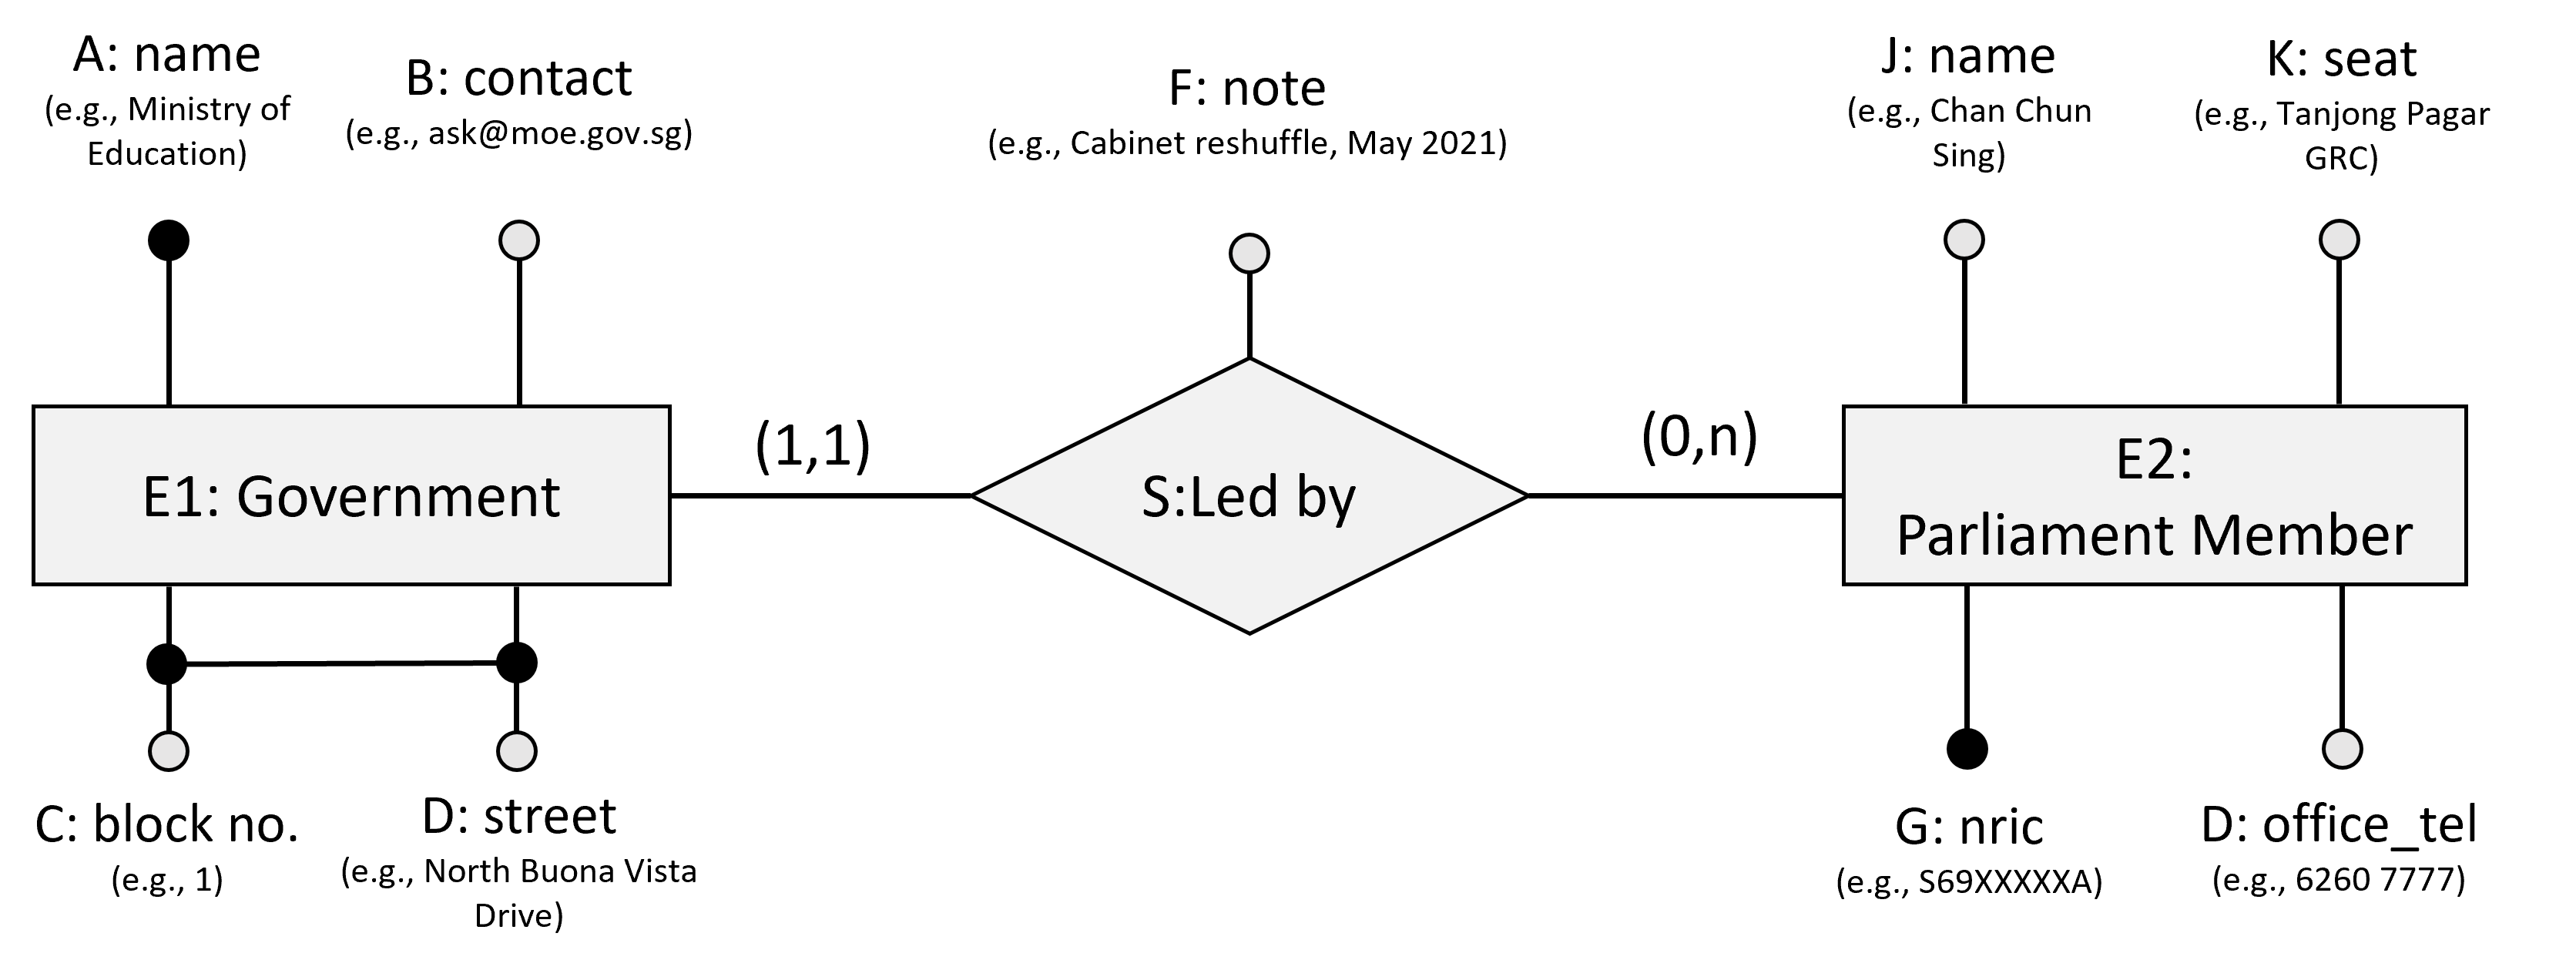
\includegraphics[width=.6\textwidth]{er.png}
		\caption{Entity-relationship diagram.}
		\label{fig:er}
	\end{center}
\end{figure}\vspace{-5pt}

\part[2] Describe in English an original real world example to which the entity-relationship diagram in Figure~\ref{fig:er} could correspond. Give the real world meaning of entity sets $E_1$ and $E_2$, of relationship set $S$, and of attributes $A$, $B$, $C$, $D$, $F$, $G$, $H$, $J$, and $K$. Justify the candidate keys and participation constraints in the entity-relationship diagram.
\begin{solution}

\begin{center}
	============ Solution provided by TA Mark Meng ============
\end{center}\vspace{5pt}

Please refer to the case that has been used in Tutorial 4, we reuse the model and propose a real-world example as shown in Fig.~\ref{fig:er}:	
\vspace{5pt}

\textbf{Candidate keys}: For E1, two candidate keys can be identified: name of the government department (A), or the composite of block number (C) and street name (D).
For E2, there is only one candidate key, which is the NRIC number of the parliament member (G).

\textbf{Participation}: As a typical commonwealth nation's cabinet, each government department (ministry level) has one and only one head, literally a (1,1) participation. The head of such government department needs be chosen from the parliament members belonging to the ruling political party. Therefore, for each parliament member, he/she may not been appointed as the head of any government department. In some cases, one parliament member can hold multiple appointments at different ministry at the same time (e.g., Minister of Law \& Minister of Home Affairs). For those reasons, the participation of E2 with regard of the relationship is (0,n).

\vspace{5pt}
\textbf{Poor examples (that should be avoided)}: \\
(1) Take non-text information as example attributes (e.g., year of founded, which is DATE);\\
(2) Take null-able information as example attributes (e.g., spouse);\\
(3) Take information has an explicit not one-to-one dependency as example attributes (e.g., number of employees, which is better to be maintained with another table);\\
(4) Take last name and first name as the composite primary key (C and D), because even the full name usually cannot identify a person.

\end{solution}
\end{parts}
\end{questions}

\begin{center}-- END OF PAPER --\end{center}

\end{document}

